
\section{Optimizing Matching Operator}
\label{sec:optimizing-matching-operator}
In this section, we focus specifically on handling the matching operator (more precisely, the graph component),
which plays a distinct role within the \spjm queries compared to the \spj queries. We discuss two main perspectives of optimizing
the matching operator: logical transformation and physical implementation. Logical transformation is
responsible for transforming a matching operator into a logically equivalent representation,
while physical implementation focuses on how the matching operator can be efficiently executed.

\subsection{Logical Transformation}
\label{sec:handling-match-operator}
We commence with an intuitive, graph-agnostic transformation before
introducing a graph-aware technique grounded on the concept of decomposition tree, which
is the key to the optimization of graph pattern matching in the literature~\cite{huge,GLogS}.

Before proceeding, we introduce the concept of pattern decomposition that decomposes $\pattern$ into two overlapping patterns, $\pattern_1$ and $\pattern_2$, with shared vertices $V_{o} = V_{\pattern_1} \cap V_{\pattern_2}$ and shared edges $E_{o} = E_{\pattern_1} \cap E_{\pattern_2}$.
Denote $\pattern = \pattern_1 \cup \pattern_2$. Under the homomorphism semantics, the matching of $\pattern$ can be represented as:

\begin{equation}
    \label{eq:join-pattern}
    \matching(\pattern) = \matching(\pattern_1) \widehat{\Join}_{V_{o}, E_{o}} \matching(\pattern_2),
\end{equation}
where $\widehat{\Join}$ is a natural join operator for joining two graph relations based on the common vertices and edges.

It is important to note that \refeq{join-pattern} is also applicable to alternative semantics, including isomorphism and non-repeated-edge~\cite{angles2017foundations}. To support these semantics, a special all-distinct operator can be applied as a filter to remove results that contain duplicate vertices and/or edges. The adoption of the all-distinct operator is compatible with all techniques in this paper.

%There are already a considerable number of research findings and solutions for the SPJ problem \cite{}.
%Given that the main difference between SPJM and SPJ lies in the matching operator, in addressing the SPJM problem, solutions from the SPJ problem can be referenced.
%In this section, we focus on the method to deal with the matching operators.
%Firstly, an intuitive method is presented and then an advanced method based on matching decomposition is proposed.
%For simplicity, the pattern graph given in matching operators are assumed to be connected in this section.

\subsubsection{Graph-agnostic Transformation}
\label{sec:intuitive-method}
If the matching operator can be transformed into purely relational operations, the \spjm query becomes a
standard \spj query, which can then be optimized using existing relational optimizers (\refsec{relational-only}). This graph-agnostic
approach is intuitive and easy to implement on top of existing relational databases, making it a straightforward
choice in prototyped systems~\cite{apache-age,DuckPGQ,DuckPGQ-VLDB}. However, there is no theoretical guarantee that
such a transformation is lossless in the context of \rgmapping (\refdef{rgmapping}). In this subsection,
we aim to bridge this gap by demonstrating the lossless transformation of the matching
operator under \rgmapping.
%Graph-agnostic methods~\cite{apache-age,DuckPGQ,DuckPGQ-VLDB} simply recast graph match operations
%as a sequence of relational operations (mainly joins and projections). This allows an \spjm query to be naively transformed into an \spj query, which then can be optimized through standard relational optimizers.

Consider a pattern graph $\pattern$ and one of its edges $e = (u_s, u_t)$. According to the definition of the matching operator (\refsec{matching-operator}), the graph edges and vertices that can be matched with $e$ must have the labels $\lab(e)$, $\lab(u_s)$, and $\lab(u_t)$. We further denote the relations corresponding to these edges and vertices via \rgmapping as $R_{\lab(e)}$, $R_{\lab(u_s)}$, and $R_{\lab(u_t)}$, respectively. Moreover, there must be total functions $\lambda_{\lab(e)}^s$ and $\lambda_{\lab(e)}^t$ for mapping tuples from $R_{\lab(e)}$ to $R_{\lab(u_s)}$ and $R_{\lab(u_t)}$, respectively. We define the following \EVjoin relational operation regarding $\lambda_{\lab(e)}^s$ as:

\begin{equation} \label{eq:ev-join}
\begin{split}
R_{\lab(e)} & \evjoin R_{\lab(u_s)} = \{(\tau_e, \tau_s) \;|\; \\
  &  \tau_e \in R_{\lab(e)} \land \tau_s \in R_{\lab(u_s)} \land \lambda_{\lab(e)}^s(\tau_e) = \tau_s\}.
\end{split}
\end{equation}

The \EVjoin regarding $\lambda_{\lab(e)}^t$ is defined analogously. Although called \EVjoin, the operation is associative like any relation join, meaning that the order in which the edge and vertex relations are joined does not affect the final result.


%Such a transformation, as indicated by the following lemma, maintains the integrity of the data and relationships, ensuring a lossless conversion process.
%The following lemma demonstrates that, in an \spjm query, the matching operation can be losslessly transformed into a sequence of purely relational operations.
We have the following lemma\footnote{Omitted proofs can be found in the full paper~\cite{full-paper}.}.

\begin{lemma}
    \label{lem:spjm-to-spj}
    Under \rgmapping, the matching operation in an \spjm query can be losslessly transformed into a sequence of relational joins involving $n$ vertex relations and $m$ edge relations.
\end{lemma}
\comment{
\begin{proof}
    Consider a pattern $\pattern_m$ of $m$ edges, where the $i$-th vertex is denoted as $u_i$, and the $i$-th edge is $e_i = (u_{s_i}, u_{t_i})$. %According to the $\rgmapping$, the corresponding relations of vertex $u_i$ and edge $e_i$ are denoted as $\relation{u_i}$ and $\relation{e_i}$, respectively. Furthermore, we have $\lambda_{e_i}^s$ and $\lambda_{e_i}^t$ to map tuples from $\relation{e_i}$ to $\relation{u_{s_i}}$, and from $\relation{e_i}$ to $\relation{u_{t_i}}$, respectively.

The proof proceeds by induction, starting with a pattern graph $\pattern_0$ with a single vertex and no edges. It is clear that $\matching(\pattern_0)$ yields a subset of vertices with label $\lab(u_0)$, which is mapped from the relation $\relation{\lab(u_0)}$ via $\rgmapping$. As a result, we have $R_0 = \gproject(\matching(\pattern_0)) = \relation{\lab(u_0)}$.

Next, consider $\pattern_1$ with one edge, $e_1 = (u_{s_1}, u_{t_1})$. Matching $\pattern_1$ is equivalent to retrieving the edge relation, together with the corresponding source and target vertices. Therefore, we have:
\[ R_1 = \gproject(M(\pattern_1)) = \relation{\lab(u_{s_1})} \evjoin \relation{\lab(e_1)} \evjoin \relation{\lab(u_{t_1})} \]

Assume that when $m = k-1$, $\gproject(\matching(\pattern_{k-1}))$ can be losslessly converted to a sequence of relational operators, resulting in the relation $R_{k-1}$. When $m = k$, we consider $\pattern_{k}$ of $k$ edges that is constructed from $\pattern_{k-1}$ by adding one more edge $e_k = (u_{s_k}, u_{t_k})$. For $\pattern_{k}$ to be connected, it must share at least one common vertex $V_o$ with $\pattern_{k-1}$. According to \refeq{join-pattern}, we have:
\[ \matching(\pattern_{k}) =  \matching(\pattern_{e_k}) \gjoin_{V_o} \matching(\pattern_{k-1}), \]
where $\pattern_{e_k}$ denotes a pattern that contains only the edge $e_k$, and $V_o$ is the common vertex shared by $\pattern_{k-1}$ and $\pattern_{e_k}$. Applying $\gproject$ to the above equation, we get:
\begin{equation*}
\begin{split}
R_k &= \gproject(\matching(\pattern_{k})) \\
    &= \widehat{\pi}_{A_1*}(\matching(\pattern_{e_k})) \Join_{V_o.attr}  \widehat{\pi}_{A_2*}(\matching(\pattern_{k-1})) \\
    &= \relation{\lab(u_{s_k})} \evjoin \relation{\lab(e_k)} \evjoin \relation{\lab(u_{t_k})} \Join_{V_o.attr} R_{k-1}
\end{split}
\end{equation*}
By induction, denoting $R'_i = \relation{\lab(u_{s_i})} \evjoin \relation{\lab(e_i)} \evjoin \relation{\lab(u_{t_i})}$, we have the matching operator losslessly converted to a sequence of relational join operations:
\begin{equation}
    \label{eq:graph-agnostic}
    \gproject(\matching(\pattern_{k})) = R'_k \Join R'_{k-1} \Join \cdots \Join R'_1 \Join R_0.
\end{equation}

We thus conclude the proof.
\end{proof}
}


%Given that edges may connect to common vertices, it's obvious that there are some redundant joins in \refeq{graph-agnostic}. Removing these redundancies results in
%a sequence of joins involving $n$ vertex tables and $m$ edge tables, as illustrated in the following example.

\begin{example}
  Given the pattern graph $\pattern$ shown in \reffig{intro-rgmapping-example}(b), the matching operation $\matching(\pattern)$ can be converted to a sequence of join operations as follows. Without loss of generality, we start from $\pattern_0$ containing only the vertex $u_{p_1}$, and we have $\relation{0} = \relationx{1}{\text{Person}}$ (note that the superscript 1 is used to differentiate relations of the same name).
  Next, we sequentially add the edges $e_1 = (u_{p_1}, u_{p_2})$, $e_2 = (u_{p_2}, u_{p_1})$, $e_3 = (u_{p_1}, u_m)$, and $e_4 = (u_{p_2}, u_m)$ to $\pattern_0$, resulting in the following relations:
  \begin{equation*}
    \begin{split}
    R'_1 &= \relationx{1}{\text{Person}} \Join_{\text{person\_id}=\text{pid1}} \relation{\text{Knows}} \Join_{\text{pid2}=\text{person\_id}} \relationx{2}{\text{Person}}, \\
    R'_2 &= \relationx{1}{\text{Person}} \Join_{\text{person\_id}=\text{pid}} \relationx{1}{\text{Likes}} \Join_{\text{mid}=\text{message\_id}} \relation{\text{Message}}, \\
    R'_3 &= \relationx{2}{\text{Person}} \Join_{\text{person\_id}=\text{pid}} \relationx{2}{\text{Likes}} \Join_{\text{mid}=\text{message\_id}} \relation{\text{Message}}.
    \end{split}
    \end{equation*}

    Finally, we have $\gproject(\matching(\pattern)) = R'_3 \Join R'_2 \Join R'_1 \Join \relation{0}$.
    Note that $\relationx{1}{\text{Person}}$ in $R'_2$, as well as $\relationx{2}{\text{Person}}$ and $\relation{\text{Message}}$ in $R'_3$, are redundant and can be safely removed from the final join. By eliminating these redundant relations, we obtain a sequence of joins involving 3 vertex relations and 3 edge relations.
\end{example}

\subsubsection{Graph-aware Transformation}
\label{sec:graph-aware}
%The graph-agnostic transformation may be inefficient because relational optimizers treat relations representing vertices and edges equally as the other relations,
%preventing the optimizer from utilizing graph-specific optimization techniques. %Furthermore, relational optimizers are known to struggle with queries containing a large number of joins, which is a common case in graph pattern matching.

We introduce a graph-aware transformation that incorporates key ideas from the literature on graph optimization. Following \refeq{join-pattern}, we can recursively decompose $\pattern$, forming a tree structure called the \emph{decomposition tree}. The tree has a root node that represents $\pattern$, and each non-leaf \emph{intermediate} node is a sub-pattern (a subgraph of the pattern) $\pattern' \subset \pattern$, which has a left and right child node, denoted as $\pattern'_l$ and $\pattern'_r$, respectively. %The condition of the intermediate pattern being induced
The leaf nodes of the tree are called \emph{Minimum Matching Components} (\mmc), correspond to nondivisible patterns directly solvable with specific physical operations
as will be introduced in~\refsec{physical-operators}. The decomposition tree naturally forms a logical plan for solving $\matching(\pattern)$, as demonstrated in \reffig{match-decomposition}. For any non-leaf node $\pattern'$, there exists a relationship $\matching(\pattern') = \matching(\pattern'_l) \gjoin \matching(\pattern'_r)$ according to \refeq{join-pattern}. The plan allows for the recursive computation of the entire pattern.

Following state-of-the-art graph optimizers~\cite{huge,GLogS}, to guarantee a \emph{worst-case optimal} execution plan~\cite{ngo2018worst}, all intermediate sub-patterns in the decomposition tree must be induced subgraphs of $\pattern$. Furthermore, \mmc is restricted to be a single-vertex pattern and a \emph{complete star}. A star-shaped pattern is denoted as $\pattern(u;V_s)$, where $u$ is the root vertex and $V_s$ is the set of leaf vertices\footnote{Edge directions between $u$ and $V_s$ are not important, and we assume they all point from $u$ to $V_s$.}. In the decomposition tree, given $\pattern' = \pattern'' \cup \pattern(u;V_s)$, $\pattern(u;V_s)$ is a complete star if and only if it is a right child and $V_s \subseteq V_{\pattern'}$, meaning that the leaf vertices of the complete star must all be common vertices for the decomposition. A single-edge pattern is a special case of a complete star. The complete star logically represents the physical operations of \expandintersect, which will be discussed in \refsec{physical-operators}. As shown in \reffig{match-decomposition}, a single-edge pattern, such as $\pattern_3$, is further decomposed into a single-vertex pattern and the pattern itself, allowing the optimizer to select from which vertex the edge can be expanded.


%The complete star is a logical representation of the physical operations of \expand~and \intersect, which are key to the implementation worst-case optimal join algorithm~\cite{mhedhbi2019optimizing} for graph pattern matching, as will be discussed in \refsec{xx}.

\comment{
Therefore, decomposing the matching operators recursively can finally result in a tree, whose leaf nodes are MMCs.
To ensure worst-case optimality, in the process of decomposition, the pattern graph of each decomposed matching operator should be an induced subgraph of $\mathcal{P}_0$.
The generated tree is called a decomposition tree and it is actually a logical plan of the matching operator.
\modify{Without loss of generality, the left-deep join order is employed on the tree.}

Then, it is crucial to identify which matching operators to treat as MMCs.
We adopt the definition of \emph{complete star} from \cite{huge}.
Specifically, suppose $\matching(GR, \mathcal{P})$ is decomposed into $\matching(GR, \mathcal{P}_1)$ $\widehat{\Join}$ $\matching(GR, \mathcal{P}_2)$, $\mathcal{P}_2$ is called a complete star iff $\mathcal{P}_2$ is a star $(v_r; \mathcal{H})$, $\mathcal{H} \subseteq E_{\mathcal{P}_1}$, and $|\mathcal{H}| \geq 2$, where $v_r$ is the root and $\mathcal{H}$ is the set of its leaf vertices.
Inspired by HUGE \cite{huge} and GLogS \cite{GLogS}, matching operators located on the right subtree of the join operator with complete stars as the pattern graphs are the MMCs in this paper.

Besides, a matching operator located on the left subtree of the join operator is an MMC iff its pattern graph is an edge (i.e., one edge and its adjacent two vertices).
}

\begin{figure}
    \centering
    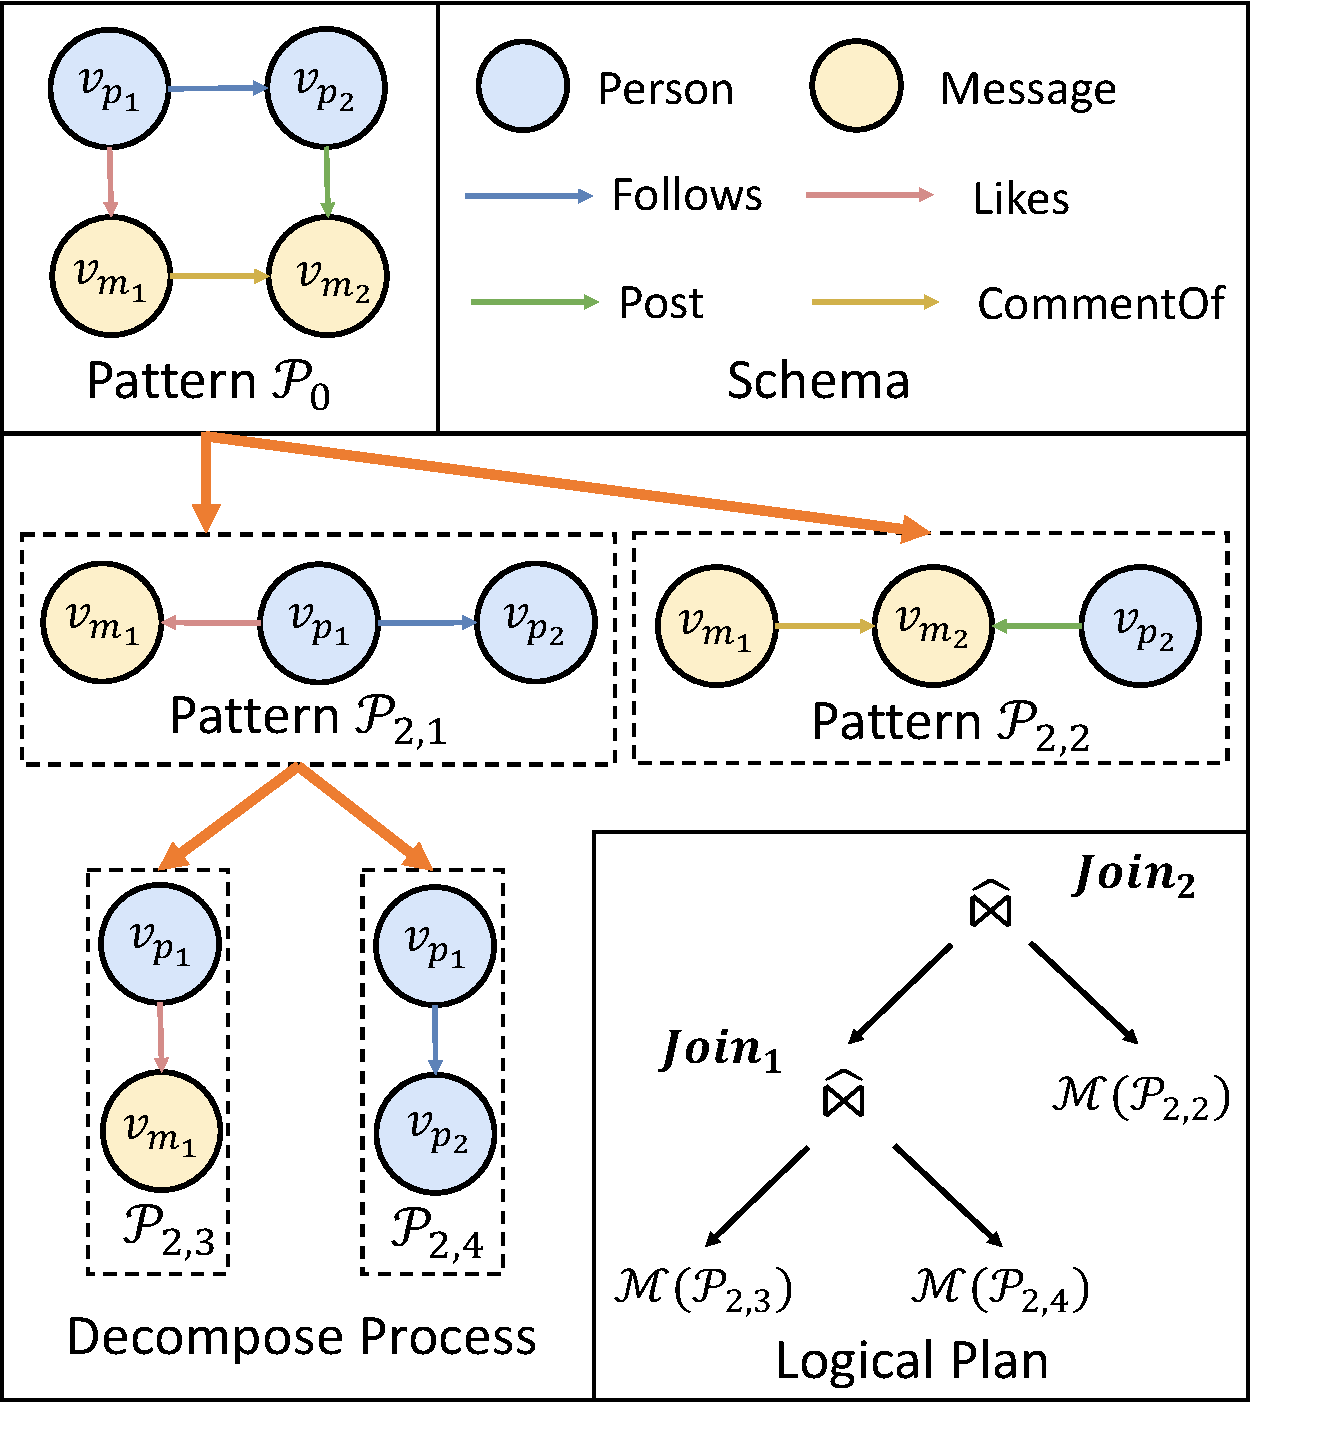
\includegraphics[width=.8\linewidth]{./figures/decomposition-example.pdf}
    \caption{Example of decomposition trees and the corresponding logical plans.}
    \label{fig:match-decomposition}
\end{figure}

\comment{
\begin{example}
    \todo{the sample and figure must all be refined.}
    \modify{
    As shown in \reffig{match-decomposition}, $T_1$ and $T_2$ are two possible decomposition trees formed by recursively decomposing $\pattern_{0}$.
    Specifically, $\pattern_{1,1}$, $\pattern_{1,3}$, $\pattern_{1,4}$, $\pattern_{2,2}$, $\pattern_{2,3}$, and $\pattern_{2,4}$ are \mmcs. Among these \mmcs, $\pattern_{1,1}$, $\pattern_{1,3}$, $\pattern_{2,3}$, $\pattern_{2,4} are $single-edge patterns, while $\pattern_{1,4}$ and $\pattern_{2,2}$ are complete stars.
    Please note that $\pattern_{2,1}$ is not an \mmc, because it is not the right child of $\pattern_{0}$.
    }
\end{example}
}

\begin{remark}
    \label{rem:graph-agnostic-vs-graph-aware}
    The graph-aware transformation is fundamentally different from its graph-agnostic counterpart. While the graph-agnostic approach consistently converts pattern matching operations into relational joins between vertex and edge relations,
    the graph-aware transformation does not, due to the constraints imposed by pattern decomposition. While the graph-agnostic approach is straightforward, it has the following drawbacks:
    \begin{itemize}
    \item \textbf{Graph-unaware Join Order}: It may cause the relational optimizer to change the order of joining vertex and edge relations, potentially missing opportunities to leverage graph indexes for the efficient computation of adjacent edges and vertices, as will be further discussed in \refsec{graph-index}.
    \item \textbf{Suboptimal Join Plans}: It generates plans that consistently reflect edge-based join plans that have been shown to be suboptimal in terms of worst-case performance~\cite{lai2015scalable}.
    \item \textbf{Increased Search Space}: Compared to the graph-aware transformation, it can lead to an exponentially larger search space when computing optimal plans, which will be elaborated upon in the following subsection.
    \end{itemize}
\end{remark}

\subsubsection{The Search Space: Graph-agnostic vs Graph-aware}
\label{sec:compare-search-space}
After applying graph-agnostic transformations to the matching operator, the optimizer searches for the optimal join order. In contrast, applying graph-aware transformations leads to a search for the optimal decomposition tree. The search space for the graph-agnostic approach is clearly larger than that of the graph-aware approach, given the constraints imposed on the decomposition tree in the latter approach. However, the precise difference in search space complexity between the two approaches has not been rigorously analyzed. In this subsection, we derive a lower bound on the search space of the graph-agnostic approach and an upper bound on the search space of the graph-aware approach to demonstrate that the letter is exponentially more efficient in terms of search space.
%Here, we argue that the comparison of the search space is general. First, some optimizers, such as the one proposed in~\cite{Haffnerjoinorder}, involve heuristics that make it challenging to perform a rigorous analysis of their behavior. Second, the abundance of relational optimizers~\cite{astarjoin,chenjoinorder, Haffnerjoinorder}, makes it difficult to select a single optimizer as the gold standard for comparison. Finally, the techniques employed by relational optimizers may also be applicable to their graph counterparts, potentially resulting in similar improvements in both cases.

According to \reflem{spjm-to-spj}, the graph-agnostic approach must produce a sequence of joins among $n$ vertex relations and $m$ edge relations,
which is equivalent to searching for the optimal join order among $n + m$ relations. The following lemma
establishes a lower bound on the search space complexity for this problem:

\begin{lemma}
\label{lem:complexity-of-volcano}
Given a join among $n + m$ relations, the search space for determining the optimal join order is at least $\Omega(4^{m+n-1})$.
\end{lemma}

\comment{
\begin{proof}
    We first estimate the number of possible join orders, where each join order corresponds to a logical plan of join operators. The search space refers to the number of physical plans corresponding to these logical plans. To avoid cross products, for each explored logical plan, whenever two relations are joined together, there should be join conditions between them.

    Given $n + m$ relations, we construct a graph $\searchgraph = (V, E)$, where each relation corresponds to a vertex in $V$, and if there is a join condition between two relations, there is an edge between their corresponding vertices in $E$. Each possible logical plan forms a spanning tree in $\searchgraph$, and different logical plans may form the same tree. Therefore, the number of possible logical plans can be computed by obtaining all the possible logical plans corresponding to the spanning trees in $\searchgraph$.

    We consider the case where there is only one spanning tree $ST$ in $\searchgraph$ with $k$ edges. When there are multiple spanning trees in $\searchgraph$, we compute the number of logical plans corresponding to one of these trees, which provides a lower bound on the total number of possible logical plans.

    First, we examine the case where $ST$ is a path. Let $c_p(k)$ denote the number of logical plans corresponding to a spanning tree that is a path of length $k$. We have:
    \begin{equation*}
        c_p(k) = 2\sum_{i=0}^{i=k-1}c_p(i)c_p(k-1-i),
    \end{equation*}
    where $c_p(0) = 1$. Using the generating function, we obtain:
    \begin{equation*}
        c_p(k) = \frac{2^k}{k+1}\binom{2k}{k} \geq \frac{2^k}{k+1}2^{k-1}(k+1) = \frac{4^k}{2}
    \end{equation*}

    Next, we consider a more general scenario where $ST$ is not necessarily a path. Let $c(ST)$ denote the number of logical plans corresponding to $ST$. Suppose there are $k$ edges in $ST$. We denote the longest path in the tree by $p_1$, with length $P_1 = |p_1|$. By removing edges in $p_1$ from $ST$, we obtain a new subgraph $ST_1$. We then find the longest path $p_2$ in $ST_1$ that intersects with the already removed path $p_1$, with length $P_2 = |p_2|$. We remove edges in $p_2$ from $ST_1$ to obtain subgraph $ST_2$. Since $p_1$ and $p_2$ are both paths, the number of logical plans corresponding to them are $c_p(P_1)$ and $c_p(P_2)$, respectively. If $p_1$ and $p_2$ intersect at vertex $v_i$, the operator that scans $v_i$ appears in each logical plan corresponding to $p_1$. By replacing these scanning operators with the plans corresponding to $p_2$, we obtain $c(p_1 \cup p_2)$ plans, satisfying $c(p_1 \cup p_2) \geq c_p(p_1)c_p(p_2)$ because the relations corresponding to vertices in $p_1$ and those in $p_2$ can be joined in an interleaved fashion, which is overlooked by multiplying $c_p(p_1)$ and $c_p(p_2)$.

    As $ST$ is a tree, by repeatedly finding and removing paths as described above, all edges in $ST$ are eventually removed. Let $s$ be the number of paths removed. We have:
    \begin{equation*}
    \begin{split}
        c(ST) & = c(p_1 \cup \cdots \cup p_s) \geq c_p(P_1) \cdots c_p(P_s) \\
        & \geq \frac{4^{P_1 + \cdots + P_s}}{2^s} = \frac{4^{k}}{2^s} \geq 2^{k}.
    \end{split}
    \end{equation*}

    Since there are $m + n$ vertices in $\mathbb{G}$, the number of edges in the spanning tree is $k = m + n - 1$. Thus, the number of physical plans is at least $2^{k}t^{m+n-1} \geq 2^{m+n-1}t^{m+n-1} \geq 4^{m+n-1}$, which is also the search space of the problem. This concludes the proof.
\end{proof}
}

In contrast, when the graph-aware transformation is applied, the search space is equivalent to the number of possible decomposition trees. Despite the numerous works proposed to optimize graph pattern matching~\cite{huge,GLogS,mhedhbi2019optimizing}, to the best of our knowledge, the search space of this optimization problem has not been thoroughly analyzed. The following lemma provides an upper bound on the search space complexity for the graph-aware approach:

\begin{lemma}
\label{lem:complexity-of-graph-aware}
The search space for determining the optimal decomposition tree for pattern $\pattern$ is at most $O(4^n)$.
\end{lemma}

\comment{
\begin{proof}
    To prove the lemma, we construct a graph $\searchgraph_\pattern(V, E)$ to facilitate the analysis, where the vertex set contains all induced sub-patterns of $\pattern$ as well as an empty graph $\pattern_{\emptyset}$.
    We denote $V_i \subseteq V$ as the set of sub-patterns that contain exactly $i \leq n$ vertices. It is evident that $V_n = \{\pattern\}$.
    An edge exists from a larger (a pattern is considered larger if it contains more vertices) sub-pattern $\pattern_1$ to a smaller sub-pattern $\pattern_2$ if it is possible for $\pattern_2$ to be the child of $\pattern_1$ in any decomposition tree. Each edge has a weight representing the cost of extending graphs matching $\pattern_2$ to those matching $\pattern_1$.
    Moreover, there are edges weighted 0 from sub-patterns in $V_1$ to $\pattern_{\emptyset}$.
    Given the graph $\searchgraph_\pattern(V, E)$, %the problem of determining the optimal decomposition tree for the graph-aware method can be transformed to finding the shortest path from $\pattern$ to $\pattern_{\emptyset}$ in $\searchgraph_\pattern(V, E)$.
    the search space equals the number of paths from $\pattern$ to $\pattern_{\emptyset}$.

    Determining the exact number of edges in $\searchgraph_\pattern$ for an arbitrary pattern is non-trivial. However, since we are studying the upper bound, we can consider the worst-case scenario. Given a sub-pattern $\pattern'$ consisting of $1 < i \leq n$ vertices, the number of induced subgraphs of $\pattern'$ with $j$ vertices is at most $\binom{i}{j}$, which constrains the maximum number of edges to $\pattern_j \in V_j$ that $\pattern'$ can connect.

    Denote the maximum number of paths from a sub-pattern with $s$ vertices (i.e., $\pattern_s \in V_s$) to $\pattern_{\emptyset}$ by $\decompnum_\pattern(s)$.
    Please note that $\decompnum_\pattern(1) = 1$ and $\decompnum_\pattern(n)$ is an upper bound of the search space for determining the optimal decomposition tree for $\pattern$.
    Then, we have the following inequality:
    \begin{equation*}
        \decompnum_{\pattern}(n) \leq \binom{n}{1}\decompnum_{\pattern}(n-1)\decompnum_{\pattern}(1) + \cdots + \binom{n}{n-1}\decompnum_{\pattern}(1)\decompnum_{\pattern}(n-1).
    \end{equation*}

    It is clear that $\decompnum_\pattern(i) \geq \decompnum_\pattern(j)$ if $i > j$.
    Therefore, we have
    \begin{equation*}
        \decompnum_{\pattern}(n) \leq \decompnumsq{2}_\pattern(n-1)(\binom{n}{1} + \cdots + \binom{n}{n-1}) < \decompnumsq{2}_\pattern(n-1)2^{n}
    \end{equation*}
    By recursively replacing $\decompnum_\pattern(n-1), \decompnum_\pattern(n-2), \cdots, \decompnum_\pattern(2)$, we can obtain the following inequalities:
    \begin{equation*}
        \begin{split}
            \decompnum_{\pattern}(n) & < (\decompnumsq{2}_\pattern(n-2)2^{n-1})^22^n = \decompnumsq{4}_\pattern(n-2)2^{n+2n-2} \\
            & < (\decompnumsq{2}_\pattern(n-3)2^{n-2})^42^{n+2n-2} = \decompnumsq{8}_\pattern(n-3)2^{n+2n-2 + 4n-8} \\
            & < \cdots \\
            & < \decompnumsq{2^{n-1}}_\pattern(1)2^{(1+\cdots+2^{n-2})n - (0+ 2 + \cdots + (n-2)2^{n-2})} < 4^{n-1}
        \end{split}
    \end{equation*}

    Therefore, the search space is at most $O(4^{n-1})$.
    We thus conclude the proof.
\end{proof}
}

\comment{
    \begin{proof}
        \todo{refine the proof.}
        Given graph $\searchgraph_\pattern(V, E)$, the problem of determining the optimal decomposition tree for the graph-aware method can be transformed to finding the shortest path from $\pattern$ to $\pattern_{\empty}$ in $\searchgraph_\pattern(V, E)$.
        According to Dijkstra's algorithm, the time complexity of the shortest path query problem is $O(|E|)$.

        As the number of edges from patterns in $V_i$ is at most
        \begin{equation*}
            \sum\limits_{\pattern_i}(2^i - 2) = \binom{n}{i}(2^i - 2),
        \end{equation*}
        the upper bound of the number of edges in $\searchgraph_\pattern$ is
        \begin{equation*}
            \begin{split}
                \sum\limits_{i=2}^{i=n}\binom{n}{i}(2^i - 2) + n
                < \sum\limits_{i=0}^{i=n}\binom{n}{i}2^i = (2+1)^n
                 = 3^n.
            \end{split}
        \end{equation*}

        Therefore, the time complexity is at most $O(3^n)$.
        We thus conclude the proof.
    \end{proof}
}

We ultimately obtain the following theorem.

\begin{theorem}
    \label{thm:compare-search-space}
    The graph-aware transformation yields a search space that is exponentially smaller than that of the graph-agnostic transformation,
    for optimizing the matching operator in an \spjm query.
\end{theorem}
\begin{proof}
    According to \reflem{complexity-of-volcano} and \reflem{complexity-of-graph-aware}, we have
    \begin{equation*}
        \frac{\Omega(4^{m+n-1})}{O(4^{n-1})} = \Omega(4^m).
    \end{equation*}
\end{proof}

\begin{remark}
    \label{rem:search-space}
    It is worth noting that the search space after applying the graph-aware transformation, as given in \reflem{complexity-of-graph-aware}, does not depend on $m$, the number of edges in the pattern. This is mainly due to the constraints imposed on the decomposition tree, which require each intermediate pattern to be an induced sub-pattern. Consequently, given any subset of vertices, enumerating edges among these vertices is not necessary. To further verify the findings in \refthm{compare-search-space}, we conducted a micro-benchmark experiment using a path graph with $n$ vertices and $n - 1$ edges. We programmed an enumerator to explore the search space of both the graph-agnostic and graph-aware approaches while varying $n$. The results, shown in \reffig{exp-search-space}, confirm the significant difference in search space size between the two approaches.
\end{remark}

%To verify the correctness of \refthm{compare-search-space}, we conduct corresponding experiments to test the size of the search space (i.e., the number of all possible physical plans or the number of decomposition trees) and the time required to traverse the entire search space when using the graph-agnostic method and the graph-aware Method.
%Specifically, we consider the case where the pattern in the matching operator consists of a path formed by $n+1$ nodes and $n$ edges.
%The experimental results are shown in \reffig{exp-compare-search-space-and-time}.

\begin{figure}[ht]
    \centering
    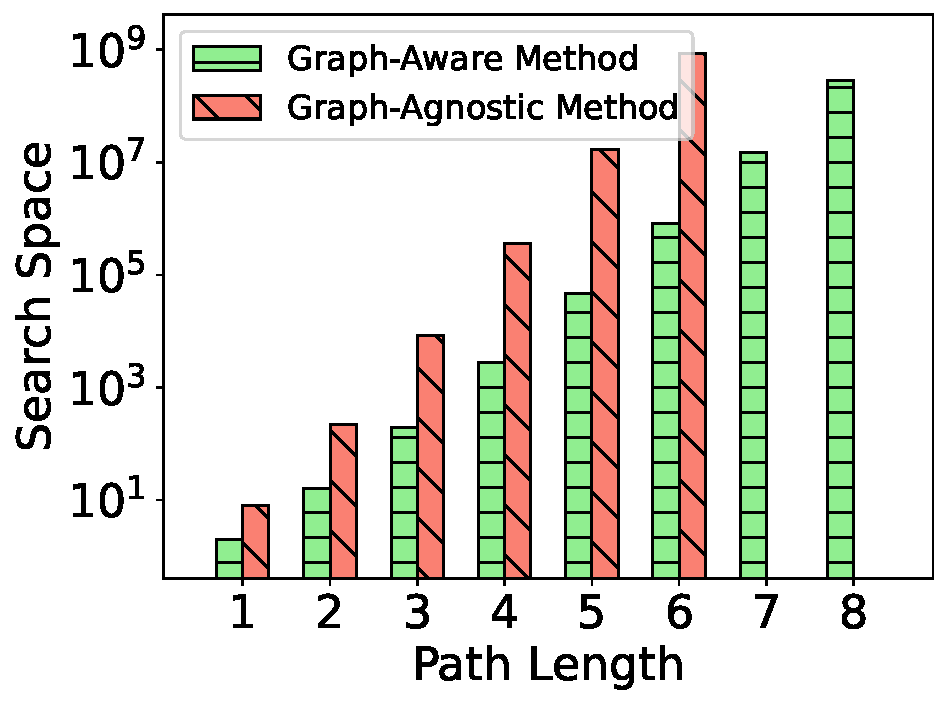
\includegraphics[width=.8\linewidth]{./figures/exp/compare_search_space.pdf}
    \caption{Search Space Comparison. Please note that when the path length is greater than 6, the memory usage of the graph-agnostic method exceeds the limit of the server with 251GB of RAM.}
    \label{fig:exp-search-space}
\end{figure}

%Please note that when the path length is greater than 6, the memory usage of the graph-agnostic method exceeds the limit.
%\reffig{exp-compare-search-space-and-time} indicate that with the increase of the number of joined relations, the search space of the both methods increase exponentially, and it is consistent with \reflem{lem:complexity-of-volcano} and \reflem{complexity-of-graph-aware}.
%Specifically, the results also demonstrate that the search space of the graph-agnostic method increase exponentially faster than that of the graph-aware method, which corroborates the correctness of \refthm{compare-search-space}.


\subsection{Physical Implementation}
\label{sec:physical-operators}

In the graph view, given a vertex $v$, it is efficient to obtain its adjacent edges and vertices (i.e., neighbors). However, in the relational view, such adjacency relationships between vertices and edges are not directly stored in relations but must be computed via the \EVjoin operations (\refeq{ev-join}). While there are multiple ways to construct the graph view in the literature~\cite{gart,GRFusion}, we refer to the method introduced in GrainDB~\cite{graindb}, which is free from materializing the graph. This approach avoids the extra storage cost associated with graph materialization and ensures compatibility with the relational context,
Specifically, GrainDB introduces an indexing technique called pre-defined join to improve the performance of join operations. As the pre-defined join essentially materializes the adjacency relationships, we treat it as a \emph{graph index} in this work.

\begin{figure}
    \centering
    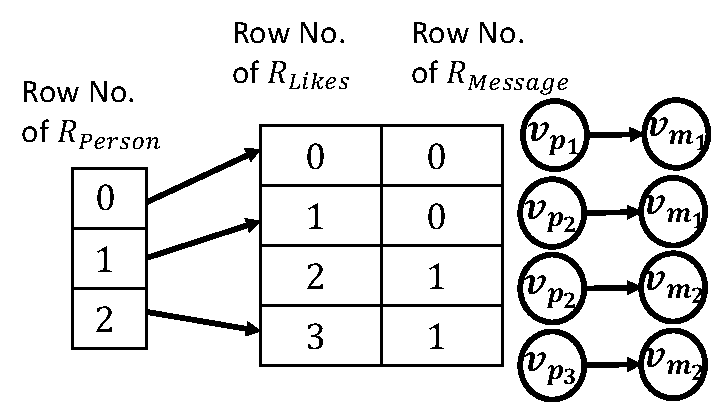
\includegraphics[width=.8\linewidth]{./figures/graph-index-likes.pdf}
    \caption{The graph index constructed among relations $\relation{\text{Person}}$, $\relation{\text{Likes}}$
    and $\relation{\text{Message}}$ in \reffig{intro-rgmapping-example}(a).}
    \label{fig:graph-index}
\end{figure}

\subsubsection{Graph Index}
\label{sec:graph-index}

As shown in \reffig{graph-index}, given the three relations $\relation{\text{Person}}$, $\relation{\text{Likes}}$, and $\relation{\text{Message}}$, the complete information of ``Person likes messages'' can be obtained by conducting the join:

\[ \relation{\text{Person}} \Join_\text{person\_id = pid} \relation{\text{Likes}} \Join_\text{mid = message\_id} \relation{\text{Message}}. \]

GrainDB introduces two kinds of indexes to the relational tables to efficiently process the join: the EV-index and the VE-index. The EV-index, shown in \reffig{graph-index}(a), is constructed by appending extra columns to the table $\relation{\text{Likes}}$. The column ``\text{pid\_rowid}'' stores the row ID of the corresponding tuple in the table $\relation{\text{Person}}$, denoted as $\rowid(\tau_{p})$, where $\tau_{p} \in \relation{\text{Person}}$. Similarly, the column ``\text{mid\_rowid}'' stores the row ID of the corresponding tuple in the table $\relation{\text{Message}}$, denoted as $\rowid(\tau_{m})$, where $\tau_{m} \in \relation{\text{Message}}$. These row ids help quickly route a tuple $\tau_{l} \in \relation{\text{Likes}}$ to the joinable tuples $\tau_{p}$ and $\tau_{m}$ without additional operations like hash-table lookup or sorting.

The VE-index, shown in \reffig{graph-index}(b), is created on the table $\relation{\text{Person}}$ for efficiently computing its ``liked messages''. For each tuple $\tau_{p} \in \relation{\text{Person}}$, the VE-index records the row ids of the tuples $\tau_{l} \in \relation{\text{Likes}}$ and the corresponding $\tau_{m} \in \relation{\text{Message}}$ that are joinable with $\tau_{p}$. In the graph view, treating ``Person-[Likes]->Messages'' as an edge of a property graph, the VE-index maintains the adjacent edges and vertices of each person. GrainDB organizes the VE-index using the Compressed-Sparse-Row (CSR) structure that is widely used for maintain adjacency lists in graph store.

We can adopt GrainDB's approach to construct the graph indexes during the \rgmapping process. Given an edge relation $R_e$ and its associated vertex relations $R_{v_s}$ and $R_{v_t}$, the EV-index can be constructed on $R_e$ for each tuple $\tau_e \in R_e$ by including $\rowid(\lambda_e^s(\tau_e))$ and $\rowid(\lambda_e^t(\tau_e))$, which are the row ids of the corresponding tuples in $R_{v_s}$ and $R_{v_t}$, respectively. Meanwhile, the VE-index can be constructed on $R_{v_s}$ for each tuple $\tau_{v_s} \in R_{v_s}$ by including the row ids of all tuples $\tau_e \in R_e$ such that $\lambda_e^s(\tau_e) = \tau_{v_s}$, along with the row ids of the corresponding tuples $\tau_{v_t} \in R_{v_t}$ such that $\lambda_e^t(\tau_e) = \tau_{v_t}$.
The construction of VE-index on $R_{v_t}$ is analogous.

\comment{
\begin{remark}
  Several alternative approaches exist for handling the \rgmapping process. One such approach, proposed in~\cite{gart}, involves directly materializing the property graph using an additional graph store, rather than simply building graph indexes on the relational data. While this method may enable more efficient graph processing, it comes with the trade-off of requiring extra storage space and incurring higher maintenance costs. Moreover, \spjm queries often involve a combination of graph and relational operations, which may not be fully supported by the graph store alone.
\end{remark}
}

%With the graph indexes constructed, we can efficiently compute the \EVjoin operation in \refeq{ev-join}.
%When using the graph-agnostic method to transform the \spjm query into \spj, as shown in \refeq{graph-agnostic}, and optimizing the entire \spj query with a relational optimizer, we can replace all the \emph{remaining} \EVjoin operations with GrainDB's pre-defined joins. This allows us to take advantage of the graph indexes provided by GrainDB. We consider this approach as the baseline ``GrainDB'' solution in our experiments.
%However, as mentioned earlier, any pair of edge and vertex relations in an \EVjoin operation can be separated during the optimization process, preventing the utilization of graph indexes.
%\modify{In \refsec{experiment-opt}, we demonstrated through experiments that using this index can be about twice as fast compared to not using the index.}
%Even if certain rules are installed to prevent such separation, the resulting plan may still be suboptimal. This is because the plan for solving the matching operator reflects a naive method of edge-based join plan~\cite{lai2019distributed}, which is not worst-case optimal. \todo{add a few experiment findings}
%\modify{Specifically, experimental results in \reffig{exp-expand-intersect} indicate that the performance of a worst-case-optimal plan can be improved by about 1.3$\times$.}

\subsubsection{The Graph-Aware Execution Plan}
\label{sec:join-matching-operator}
We delve into the physical implementation of the execution plan provided by the graph-aware method for solving $\matching(\pattern)$. The entry point of the plan is always matching a single-vertex pattern $\pattern_u$, which is one of the leaf nodes in the decomposition tree.

 The implementation of $\matching(\pattern_u)$ is straightforward: scanning the corresponding vertex relation $\relation{\lab(u)}$ and encoding each tuple as a graph vertex object that contains its ID and label (mandatory) and necessary attributes. The row ID of the tuple in the relation can be directly used as the ID. To ensure globally uniqueness, the name of the relation can be incorporated as a prefix of the ID. Advanced encoding techniques are necessary for production use, but they are beyond the scope of this paper.

The plan is then constructed in a bottom-up manner. As shown in \reffig{match-decomposition}, there are three fundamental cases to consider when implementing the plan.

\stitle{Case I: Solving $\matching(\pattern') = \matching(\pattern'_l) \gjoin_{V_o, E_o} \matching(\pattern'_r)$}, where $\pattern_l'$ and $\pattern'_r$ are both intermediate patterns in the decomposition tree. The implementation of such a join is similar to a conventional relational join. The join is constrained to a natural join, where the join condition is simply the equality of the common vertices $V_o$ and edges $E_o$ between $\pattern_l'$ and $\pattern_r'$. During the implementation of the join, the identifiers of the vertices and edges can serve as the keys for comparison. Note that the input and output of the join are both graph relations, which will not
be projected into relational tuples until the last stage that obtains the results $\matching(\pattern)$.

\stitle{Case II: Solving $\matching(\pattern') = \matching(\pattern'_l) \gjoin_{u_s} \matching(\pattern_e)$}, where $\pattern_e$ is a single-edge pattern, and $u_s$ is the source vertex in $\pattern'_l$ from which the edge $e = (u_s, u_t)$ is expanded. Note that it's not possible for both $u_s$ and $u_t$ to be in $\pattern'_l$, as it would violate the fact that $\pattern'_l$ is either a single vertex or an induced sub-pattern.

When there is no graph index, the results of $\matching(\pattern_e)$ are computed via $R_{\lab(u_s)} \evjoin R_{\lab(e)} \evjoin R_{\lab(u_t)}$,
where the first join is to obtain the edge tuples that connect $u_s$, which are encoded into edge objects,
and the second join is to obtain the associated vertex tuples of $u_t$, which are encoded into vertex objects.
%following the encoding of vertex tuples into vertex objects and edge tuples into edge objects.
This case is then reduced to Case I, where a join operation is performed between $\matching(\pattern'_l)$ and the computed $\matching(\pattern_e)$.

When graph indexes exist, the implementation is handled by the physical operators of \expandedge~ and \getvertex. For each tuple $\tau \in \matching(\pattern'_l)$, $\tau.u_s$ must record a graph vertex $v_s$ that matches $u_s$ in the pattern $\pattern'_l$. The \expandedge~ operator looks up the VE-index of $v_s$, which allows it to efficiently computes $v_s$'s adjacent edges (more precisely, it's the corresponding edge tuples). Furthermore, the \getvertex~ operator is used to obtain the matched vertex $v_t$ that is connected to $v_s$ via the previous matched edges, which can be achieved by looking up the EV-index of the matched edges.
By combining the results of \expandedge~ and \getvertex, the tuple of $(\tau, \adj^E(v_s), \adj(v_s))$ is rendered. For example, in \reffig{graph-index}(b), if we apply \expandedge~ and \getvertex~ to a tuple $\tau$ from $v_{p_2}$, the result $(\tau, [e_{l_2}, e_{l_3}], [v_{m_1}, v_{m_2}])$ is returned.
Furthermore, to obtain $\matching(\pattern')$, we flatten the adjacent edges and vertices and pair them up. In the case of $(\tau, [e_{l_2}, e_{l_3}], [v_{m_1}, v_{m_2}])$, two tuples $(\tau, e_{l_2}, v_{m_1})$ and $(\tau, e_{l_3}, v_{m_2})$ are generated.

In real-life scenarios, a vertex may be adjacent to multiple types of edges. For example, in \reffig{intro-rgmapping-example}, a \kk{Person} vertex can be connected to both \kk{Likes} and \kk{Knows} edges. To handle such cases, we can record edge's ID instead of just the row ID of the tuple. Given that the edge's ID is a combination of its label and the tuple's row ID, the adjacent edges of a specific label can be easily obtained from the VE-Index.

\stitle{Case III: Solving $\matching(\pattern') = \matching(\pattern'_l) \gjoin_{V_s, E_s} \matching(\pattern(u;V_s))$}, where $\pattern(u;V_s)$ is a complete $k$-star pattern. In this case, $\pattern'_l$ is a sub-pattern, and $\pattern(u;V_s)$ is a complete $k$-star pattern with a root vertex $u$ and leaf vertices $V_s = \{u_1, \ldots, u_k\}$.

When there is no graph index, solving Case III involves continuously joining $|V_s|$ single-edge patterns.

When graph indexes are available, we can use the \expandintersect~ operator, introduced in the literature~\cite{huge,GLogS,mhedhbi2019optimizing}, to efficiently compute the join. Given a tuple $\tau \in \matching(\pattern'_l)$, let $\{v_1, \ldots, v_k\}$ be the vertices in $\tau$ that match the leaf vertices $\{u_1, \ldots, u_k\}$ in the complete star $\pattern(u;V_s)$. The vertices that can match the root vertex $u$ of the star must be the common neighbors of all the leaf vertices.

Consequently, for the tuple $\tau$, the physical \expandintersect~ operator performs the following steps:

\begin{enumerate}
\item For each leaf vertex $u_i \in V_s$, where $1 \leq i \leq k$, apply the \expandedge~ and \getvertex~ operators to obtain the adjacent edges and neighbors of the corresponding vertices $v_i$ respectively.
\item Compute the intersections of all adjacent edges and neighbors returned by the \expandedge~ and \getvertex~ operators.
\item Return a new tuple as follows, where the information of edges is ommited for simplicity.
%\[
%    \left(\tau,\bigcup\limits_{v_c \in \bigcap\limits_{1 \leq i \leq k} \adj(v_i)} (v_c, \bigcup\limits_{1 \leq i \leq k}\adj^E(v_i, v_c))\right)
%\]
\[
    (\tau, \bigcap_{1 \leq i \leq k}\adj(v_i)).
\]

\end{enumerate}

Note that the above step (1) and (2) can be computed in a pipeline manner, following a certain order of among the leaf vertices.
Similar to Case II, we flatten the common edges and vertices and pair them up to obtain the final result.

\begin{example}
    \todo{should better refactor the example using Figure 5, by also drawing the physical plan in Figure 5}
    \todo{moreover, combining Figure 5/6 may be a good idea.}
    Given $\pattern_0$ in \reffig{match-decomposition}, a decomposition tree and the corresponding logical plan is presented.
    The implementation of the decompostion tree follows a bottom-up order.
    Firstly, the join operation between $\matching(\pattern_5)$ and $\matching(\pattern_6)$ is implemented and it pertains to Case II, since the $\pattern_6$ is a single-edge pattern.
    Thus, when there is no graph index on $\relation{Likes}$, the results of $\matching(\pattern_6)$ is computed via $\relation{Message} \Join_{message\_id = mid} \relation{Likes} \Join_{pid = person\_id} \relation{Person}$.
    Then, since $\pattern_5$ is a single-vertex pattern whose vertex exists in $\pattern_6$, the results of the join equals $\matching(\pattern_6)$.
    Otherwise, if a graph index exists, $\matching(\pattern_6)$ can be computed with \expandedge~and \getvertex.
    Analogously, the join operation between $\matching(\pattern_7)$ and $\matching(\pattern_8)$ also pretains to Case II.
    
    Then, $\matching(\pattern_3) \widehat{\Join}_{\{u_{p_1}\}} \matching(\pattern_4)$ pretains to Case I.
    The join operator is implemented as a natural join with constraints on $u_{p_1}$.

    Finally, $\matching(\pattern_1)$ and $\matching(\pattern_2)$ are joined together, where $\pattern_2 = (u_{m_2}, \{u_{m_1}, u_{p_2}\})$ is a complete $2$-star pattern.
    For simplicity, suppose $(v_{m}, v_{p}, v_p')$ is a tuple in $\matching(\pattern_1)$, where $v_{m}, v_{p}, v_p'$ are vertices that matches $u_{m_1}$, $u_{p_2}$, and $u_{p_1}$ respectively.
    $\adj(v_{m})$, $\adj(v_{p})$ are neighbors of $v_m$ and $v_p$ labeled Message.
    Suppose the graph indexes are available, the physical operator \expandintersect~is applied.
    Specifically, \expandedge~and \getvertex~operators are applied to obtain the adjacent edges and neighbors of $v_m$ and $v_p$, and the obtained tuples are $(v_m, \adj(v_m))$ and $(v_p, \adj(v_p))$.
    Then, these two tuples are intersected and a new tuple $(v_m, v_p, \adj(v_m) \cup \adj(v_p))$ is obtained.
    Finanlly, this tuple is concatenated with $\tau$ and tuple $(v_m, v_p, v_p', \adj(v_m) \cup \adj(v_p))$ is returned.
    This returned tuple can be flattened if necessary.
\end{example}
